\chapter{About the author}

\begin{wrapfigure}{R}{0.33\textwidth}
    \centering
    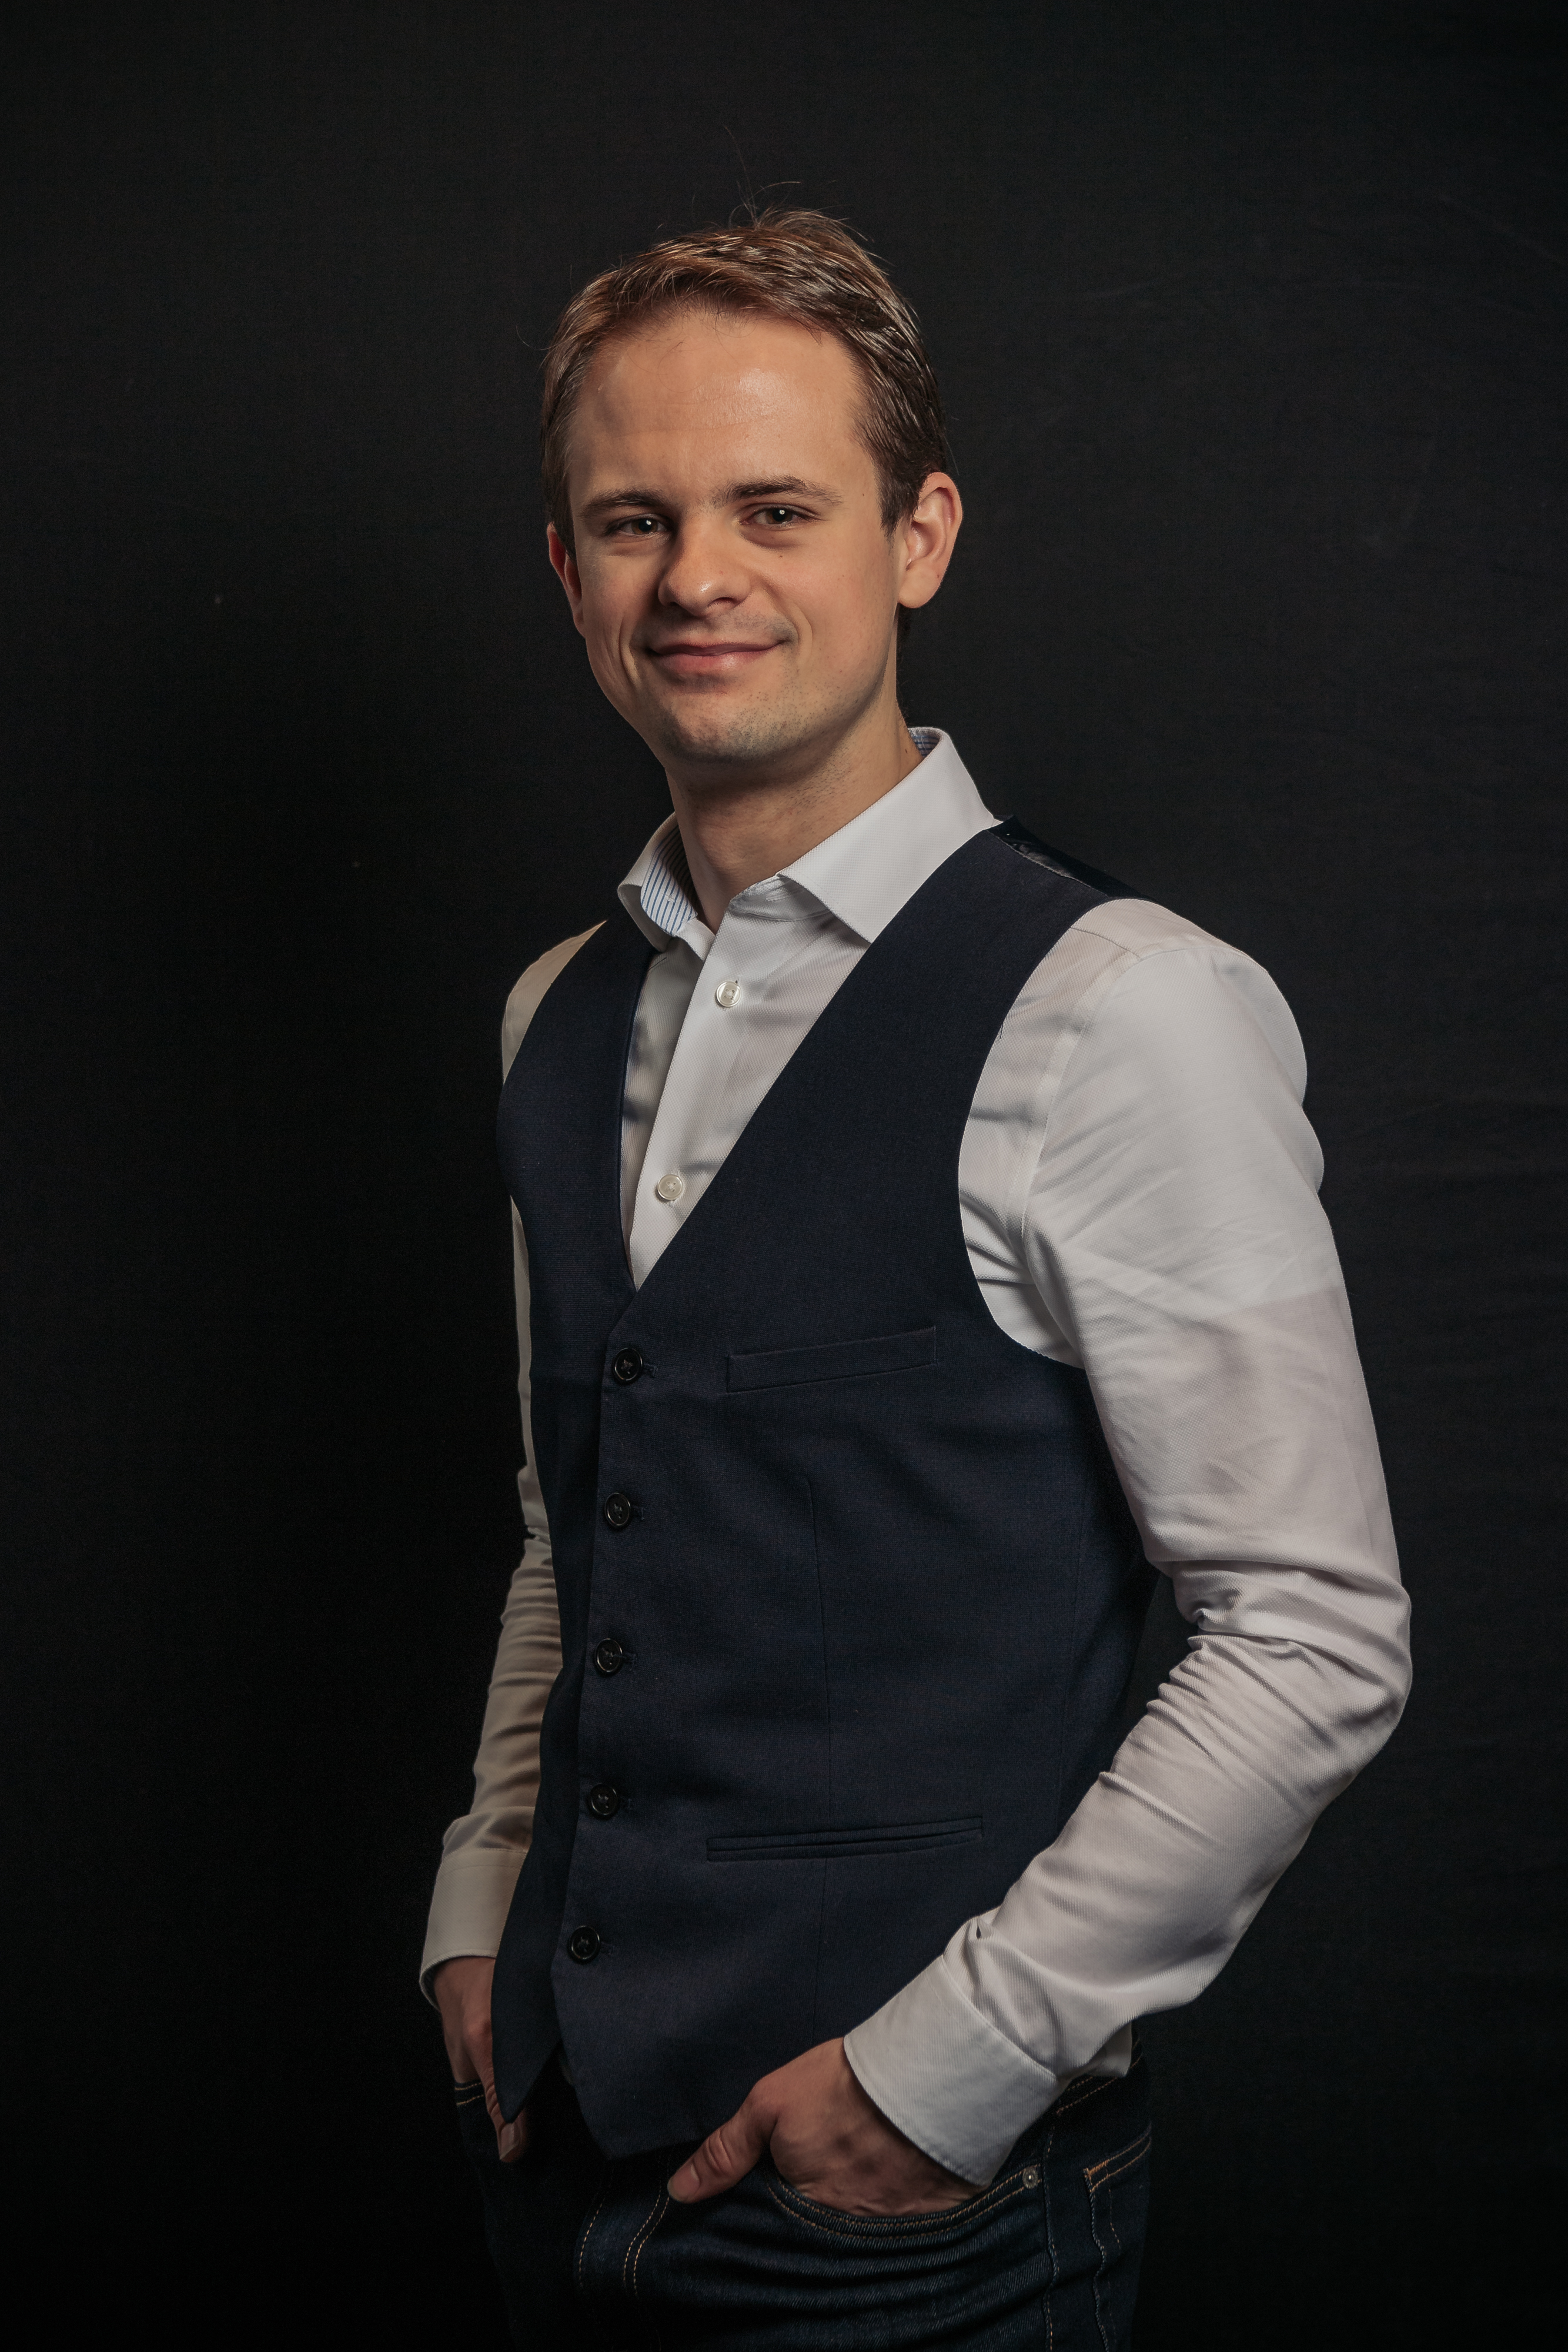
\includegraphics[width=0.3\textwidth]{Figures/Picture_Sebastian_van_der_Voort_full.jpg}
\end{wrapfigure}


Sebastian Robert van der Voort was born in Leidschendam, The Netherlands on the 30th of December 1991.
In 2010 he finished high school in The Hague, and started a Bachelor of Applied Physics at the Delft University of Technology.
After successfully completing his Bachelor in 2013 he continued with his Master of Applied Physics at the same university, with the specialization Nuclear Science and Engineering.
He finished his Master in 2015 with the predicate \say{Cum Laude}.
In his MSc thesis, Sebastian focused on designing a more efficient proton therapy dose calculation.

\vspace{\baselineskip}
\noindent After finishing his Master, Sebastian started his PhD at the Biomedical Imaging Group Rotterdam (BIGR), Erasmus MC, in June 2016.
The PhD project was entitled \say{Noninvasive phenotyping of molecular brain tumour profiles using novel advanced MR imaging and analysis}.
He was supervised by Marion Smits (promoter), Wiro Niessen (promoter), and Stefan Klein (co-promoter).
Sebastian investigated the application of machine learning methods for the image analysis of glioma MRI scans.
He developed several methods that can predict the genetic and histological features of glioma from pre-operative scans, and investigated potential imaging markers.
During his PhD he was also active in several associations that promote the opportunities of clinical technology to a wider audience.
